\documentclass[varwidth=true, border=2pt]{standalone}
\usepackage{tikz}
\usetikzlibrary{shapes, calc, shapes, arrows} 
\usepackage{amsmath,amssymb}

\usepackage{xcolor}
\definecolor{xvectorcolor}{HTML}{77933C}

\begin{document}
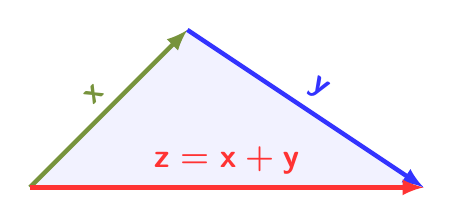
\begin{tikzpicture}[font=\boldmath]\large
    % Punkte
    \coordinate (A) at (0,0) {};
    \coordinate (B) at (5,0) {};
    \coordinate (C) at (2,2) {};

    % Draw the triangle
    \path[fill=blue!10, fill=blue!5]  (A) -- (B) -- (C) -- (A);
    \draw[->, ultra thick, xvectorcolor, arrows={-latex}]  (A) -- (C) node[sloped,midway,above] {$\mathsf{x}$};
    \draw[->, ultra thick, blue!80,      arrows={-latex}]  (C) -- (B) node[sloped,midway,above] {$\mathsf{y}$};
    \draw[->, ultra thick, red!80,       arrows={-latex}]  (A) -- (B) node[sloped,midway,above] {$\mathsf{z = x+y}$};
    %\coordinate  (A) -- (B) node[sloped,midway,below] {$\mathsf{\|z\| = \|x+y\| \leq \|x\| + \|y\|}$};
\end{tikzpicture}
\end{document}
